Algoritmi opisani u ovom radu se mogu relativno jednostavno implementirati u bilo kojem modernom programskom jeziku. Zapravo, najve\cj i problem predstavlja \ch itanje i pisanje video datoteka. Naime,
za to nam je potreban na\ch in da pozovemo odgovaraju\cj i \textit{codec} (eng. \textit{coder-decoder}) za format video datoteke koji koristimo. OpenCV biblioteka nam omogu\cj ava upravo \ch itanje
i pisanje video datoteka, te direktan pristup pikselima svakog frejma, \sh to je nama od klju\ch nog zna\ch aja za svaki opisani algoritam.

\section{OpenCV} %http://opencv.org/about.html
OpenCV (eng. \textit{Open Computer Vision} je biblioteka originalno razvijena od strane Intel-a, koja se fokusira na oblasti ra\ch unarske vizije i ma\sh inskog u\ch enja. Originalna implementacija biblioteke
je u C++ programskom jeziku, dok tako\dj er postoji podr\sh ka za C, Java, Python i MATLAB. Funkcionalnosti biblioteke koje su nama potrebne uklju\ch uju \ch itanje i pisanje video datoteka sa punom
kontrolom nad atributima (poput formata, rezolucije, framerate-a, itd.), direktna kontrola nad pikselima svakog pojedina\ch nog frejma, pronala\zh enje opti\ch kog toka kroz ugra\dj ene funkcije, te neke
druge funkcionalnosti poput mogu\cj nosti prikazivanja bilo kojeg frejma na ekranu u bilo koje vrijeme. Sve ovo predstavlja jedan veoma mali dio mogu\cj nosti biblioteke, koja ima preko 2500 implementiranih
i optimizovanih algoritama, zbog \ch ega je kori\sh tena u mnogim od najve\cj ih tehnolo\sh kih kompanija na svijetu\cite{opencvabout}.

Tri najva\zh nije OpenCV klase koje \cj emo koristiti za implementaciju su \lstinline{cv::Mat}, \lstinline{cv::VideoCapture}, te \lstinline{cv::VideoWriter}. Sve klase i funkcije OpenCV biblioteke koje \cj emo mi koristiti
 se nalaze u \lstinline{cv}
imenskom prostoru\cite{cvdocs}. \lstinline{cv::Mat} je vi\sh enamjenska klasa koju OpenCV koristi za dr\zh anje raznih tipova matrica, pri \ch emu svaki element mo\zh e imati jedan ili vi\sh e razli\ch itih kanala. O\ch igledna
korist ovoga jeste da mo\zh emo istu klasu koristiti za dr\zh anje frejmova u boji (gdje svaki piksel ima 3 kanala) i samo intenziteta svakog piksela. Na primjer, ako imamo varijablu \lstinline{frejm} koja je tipa
\lstinline{cv::Mat}, da bismo pristupili vrijednosti piksela u boji na koordinatama $(x,y)$, koristimo sljede\cj i kod:
\begin{lstlisting}
cv::Vec3b piksel = frejm.at<cv::Vec3b>(y, x);
\end{lstlisting}

Pri tome, \lstinline{cv::Vec3b} je klasa koja dr\zh i tri bajta (jedan za svaki kanal), kojima mo\zh emo pristupiti kori\sh tenjem subscript operatora \lstinline{piksel[0]}, \lstinline{piksel[1]} i \lstinline{piksel[2]}. 
I \lstinline{.at} metoda i subscript operator vra\cj aju reference, tako da je isti pristup mogu\cj e koristiti i za postavljanje vrijednosti piksela, bilo \ch itavih ili pojedina\ch nih komponenti. 
Jo\sh\ treba napomenuti da subscript operatori ne referenciraju kanale piksela uobi\ch ajnim RGB (crvena-zelena-plava) redoslijedom, nego obrnutim (BGR). \lstinline{cv::Mat} tako\dj er ima \lstinline{.rows} i 
\lstinline{.cols} atribute, koji sadr\zh e broj redova odnosno broj kolona frejma (drugim rije\ch ima, rezoluciju).

\lstinline{cv::VideoCapture} i \lstinline{cv::VideoWriter} klase koristimo za \ch itanje odnosno pisanje video datoteka. Pri tome, \lstinline{cv::VideoCapture} mo\zh e uzimati video podatke i iz drugih izvora,
poput web kamera. U oba slu\ch aja, \lstinline{.open} metoda se koristi za otvaranje datoteke za \ch itanje odnosno pisanje (pri \ch emu u slu\ch aju pisanja tako\dj er navodimo potrebne informacije poput
formata, rezolucije, i framerate-a video zapisa), tok se \lstinline{.release} koristi za pravilno zatvaranje. \lstinline{cv::VideoCapture} implementira \lstinline{.read} metodu, ili ekvivalentni \lstinline{>>} operator koji
pro\ch ita, dekodira, i vrati naredni nepro\ch itani frejm (vrijednost tipa \lstinline{cv::Mat}. Da bismo znali da smo do\sh li do kraja video zapisa, preporu\ch eni na\ch in jeste poziv metode \lstinline{.empty()} 
nad vra\cj enim frejmom, koja \cj e vratiti logi\ch ku vrijednost \lstinline{true} ako smo ve\cj\ pro\ch itali posljednji frejm video zapisa, zbog \ch ega \cj e svaki drugi poku\sh aj \ch itanja rezultirati praznim frejmom.

Prate\cj i istu logiku, \lstinline{cv::VideoWriter} implementira \lstinline{.write} metodu, umjesto koje mo\zh emo koristiti \lstinline{<<} operator. Parametar u oba slu\ch aja predstavlja vrijednost tipa
\lstinline{cv::Mat}, koja \cj e biti dodana na kraj video zapisa. Pozivom prije spomenute metode, video zapis \cj e biti zapisan u datoteku. Ako parametri proslije\dj eni konstruktoru \lstinline{cv::VideoWriter}
objekta ne odgovaraju formatu frejmova koje poku\sh avamo dodati u video zapis, napravljena datoteka \cj e biti veli\ch ine svega nekoliko kilobajta i ne\cj e sadr\zh avati nikakve korisne informacije.
Treba imati na umu da \lstinline{cv::VideoWriter}, kroz ovakvu "direktnu" upotrebu, ne\cj e ubaciti audio zapis u video datoteku. To je za o\ch ekivati, jer nismo audio zapis nigdje ni naveli.

% Dodati Farneback-a, ako bude koristen

\section{Implementacija}
Osnovni tok interpolatora je sljede\cj i\cite{implementation}:
\begin{enumerate}
\item Inicijaliziraj objekte za \ch itanje i pisanje video datoteka
\item U\ch itaj prethodni frejm
\item U\ch itaj naredni frejm
\item Ako je naredni frejm prazan, zavr\sh i sa radom
\item Inicijaliziraj objekat za pronala\zh enje opti\ch kog toka, te pozovi metodu za izvr\sh avanje
\item Prona\dj eni opti\ch ki tok proslijedi metodi za generaciju interpoliranog frejma
\item Pro\dj i kroz svaki piksel i na osnovu opti\ch kog toka odredi poziciju u interpoliranom frejmu
\item Pozovi metodu koja popravlja "rupe" u frejmu
\item Popravi gre\sh ke opisane u poglavlju 4
\item Novi frejm upi\sh i u video zapis
\item Zamijeni prethodni i naredni frejm (tako da \cj e prija\sh nji prethodni frejm biti prebrisan)
\item Vrati se na korak 3
\end{enumerate}

Najvi\sh i nivo koda interpolatora se nalazi u \lstinline{Interpolator::run} metodi:
\begin{lstlisting}
void Interpolator::run()
{
    // Provjera ispravnosti opcija
    if (input_file_name.empty())
        throw std::logic_error("Input file name not present");
    if (output_file_name.empty())
        throw std::logic_error("Output file name not present");
    if (interpolator_options.frames_to_generate < 1)
        throw std::domain_error("frames_to_generate has to be at least 1");
        
    // Ucitavanje i postavljanje informacija o video zapisu   
    video_capture.open(input_file_name);
    video_info.fourcc = (int)video_capture.get(CV_CAP_PROP_FOURCC);
    video_info.fps = (int)video_capture.get(CV_CAP_PROP_FPS);
    video_info.height = (int)video_capture.get(CV_CAP_PROP_FRAME_HEIGHT);
    video_info.width = (int)video_capture.get(CV_CAP_PROP_FRAME_WIDTH);
    video_info.frame_count = (int)video_capture.get(CV_CAP_PROP_FRAME_COUNT);
    known_pixel_map = 
    std::vector<std::vector<char> >(video_info.height, std::vector<char>(video_info.width, 0));

    total_frames = video_info.frame_count;
    frames_processed = 0;

    // Otvaranje cv::VideoWriter objekta
    video_writer.open(output_file_name, 
                      CV_FOURCC('H', '2', '6', '4'),
                      video_info.fps * 
                      (interpolator_options.frames_to_generate + 1), 
                      cv::Size(video_info.width, video_info.height));
    if (!video_writer.isOpened())
        throw std::logic_error("Can\'t open video writer!");

    // Glavna petlja
    while (true)
    {
        if (previous_frame.empty())
        {
            video_capture >> previous_frame;
            video_capture >> next_frame;

            if (previous_frame.empty() || next_frame.empty())
                throw std::logic_error("Problem with video, stopping");
        }
        else
        {
            std::swap(previous_frame, next_frame);
            video_capture >> next_frame;

            if (next_frame.empty())
            {
                video_writer << previous_frame;
                return; 
            }
        }

        // Poziv funkcije za generisanje novih frejmova
        generate_intermediate_frames();
        video_writer << previous_frame;

        for (const auto& interpolated_frame : interpolated_frames)
            video_writer << interpolated_frame;
    }
}
\end{lstlisting}

\lstinline{CV_FOURCC('H', '2', '6', '4')} je macro za specifickaciju tzv. \textit{FOURCC} tipa video formata. H.264 je veoma popularan format, tako da interpolator sve video zapise spa\sh ava tako.
Naredni isje\ch ak koda se poziva ako \zh elimo prona\cj i opeti\ch ki tok dijamantnom pretragom:
\begin{lstlisting}
Optical_flow_field& Diamond_search::calculate()
{
    if (cost_map.empty())
        reset_cost_map();
    if (opt_flow_field.data.empty())
        init_opt_flow_field();

    for (int block_start_y = 0; block_start_y < prev_frame->rows; block_start_y += block_size)
    {
        for (int block_start_x = 0; block_start_x < prev_frame->cols; block_start_x += block_size)
        {
            Vec2 block_opt_flow = calculate_block_opt_flow({block_start_x, block_start_y});

            for (int pixel_offset_y = 0; pixel_offset_y < block_size; pixel_offset_y++)
            {
                for (int pixel_offset_x = 0; pixel_offset_x < block_size; pixel_offset_x++)
                {
                    int row = block_start_y + pixel_offset_y;
                    int col = block_start_x + pixel_offset_x;

                    if (row >= prev_frame->rows || col >= prev_frame->cols)
                        continue;

                    opt_flow_field.data[row][col] = block_opt_flow;
                }
            }
        }
    }

    return opt_flow_field;
}
\end{lstlisting}

\lstinline{Vec2} je klasa koja samo sadr\zh i dva cjelobrojna atributa. Vidimo upravo \lstinline{for} petlje koje prolaze kroz svaki blok u frejmu, te nakon izra\ch unavanja opti\ch kog toka, svaki piksel
u bloku, dodjeljuju\cj i svakom izra\ch unati vektor pomaka.

Linija koda u kojoj se izra\ch unava krajnja pozicija piksela u interpoliranom frejmu:
\begin{lstlisting}
Vec2 projected_position = Vec2(j, i) + (opt_flow_field.data[i][j] *
                    (((double)frame_idx + 1) / (interpolator_options.frames_to_generate + 1)));
\end{lstlisting}

\lstinline{Vec2(j,i)} je pozicija od koje kre\cj emo, tj. pozicija piksela u prethodnom frejmu. \lstinline{opt_flow_field.data[i][j]} je objekat tipa \lstinline{Vec2} koji predstavlja vektor pomaka za trenutni
piksel. Vektor pomaka pomno\zh imo sa faktorom koji zavisi od pozicije frejma izme\dj u dva originalna. Npr. ako izme\dj u svaka dva frejma generi\sh emo 3 dodatna, a trenutno generi\sh emo
prvog od njih, taj faktor \cj e iznositi 0.25. Taj rezultat dobijemo ako u formulu uvrstimo vrijednosti \lstinline{frame_idx = 0}, \lstinline{interpolator_options.frames_to.generate = 3}.

Klasa \lstinline{Interpolator} je glavna klasa kori\sh tena za implementaciju, te jedina \ch iju instancu moramo koristiti da bismo generisali novi video zapis. Klasa \lstinline{Optical_flow_calculator}
je apstraktna klasa koja je osnova za bilo koju klasu koju koristimo za izra\ch unavanje opti\ch kog toka. \lstinline{Optical_flow_calculator} tako\dj er sadr\zh i dodatne pomo\cj ne funkcije, poput
\lstinline{is_legal} koja provjerava da li su koordinate piksela validne, te \lstinline{grayscale_pixel}, koja vra\cj a intenzitet piksela prostom aritmeti\ch kom sredinom njegovih komponenti.
Glavna metoda je \lstinline{calculate}, koja je \ch isto virtualna, te je trebaju implementirati izvedene klase. \lstinline{calculate} vra\cj a referencu na izra\ch unati opti\ch ki tok, \sh to nam omogu\cj ava
kori\sh tenje opti\ch kog toka bez kopiranja, \sh to bi usporilo izvr\sh avanje. To tako\dj er zna\ch i da ne smijemo dopustiti da objekat bude izbrisan dok imamo referencu na opti\ch ki tok.
Sam opti\ch ki tok je sadr\zh an u \lstinline{Optical_flow_field} objektu, \ch iji atributi uklju\ch uju dimenzije polja opti\ch kog toka (radi lak\sh eg pristupa), te same podatke sa\ch uvane kao tip
\lstinline{std::vector<std::vector<Vec2>>}, odnosno jedan \lstinline{Vec2} po pikselu. Razlog za\sh to metoda \lstinline{calculate} vra\cj a referencu a ne \lstinline{const} referencu jeste \sh to \cj e
opti\ch ki tok biti kasnije izmijenjen u metodama za korekciju, kori\sh tenjem ve\cj\ obra\dj enih algoritama.

\section{Qt} %https://wiki.qt.io/About_Qt
Qt framework, razvijen 1990-ih od strane dvojice Norve\sh kih programera, je jedan od najpopularnijih GUI (eng. \textit{Graphical User Interface}) framework-a za C++ programski jezik (s tim da je
Qt dostupan i za druge jezike). Omogu\cj ava jednostavan razvoj korisni\ch kih su\ch elja, koriste\cj i najpopularnije i naj\ch e\sh \cj e kori\sh tene kontrole, poput dugmadi (\lstinline{QPushButton}),
unosa teksta (\lstinline{QLineEdit}), indikatora napretka (\lstinline{QProgressBar}), i mnogih drugih. Qt je izabran zbog svoje jednostavnosti, popularnosti, te \ch injenice da je napisan u C++-u.
Ako koristimo Qt framework, najlak\sh e nam je koristiti Qt-evo razvojno okru\zh enje, Qt Creator, koje nam omogu\cj ava pravljenje korisni\ch kih su\ch elja koriste\cj i obi\ch ni drag-drop pristup,
te je integrisano sa Qt bibliotekama, \sh to zna\ch ajno olak\sh ava razvoj\cite{qtabout}.
\begin{figure}[H]
\caption{Izgled Qt Creator-a sa otvorenim projektom}
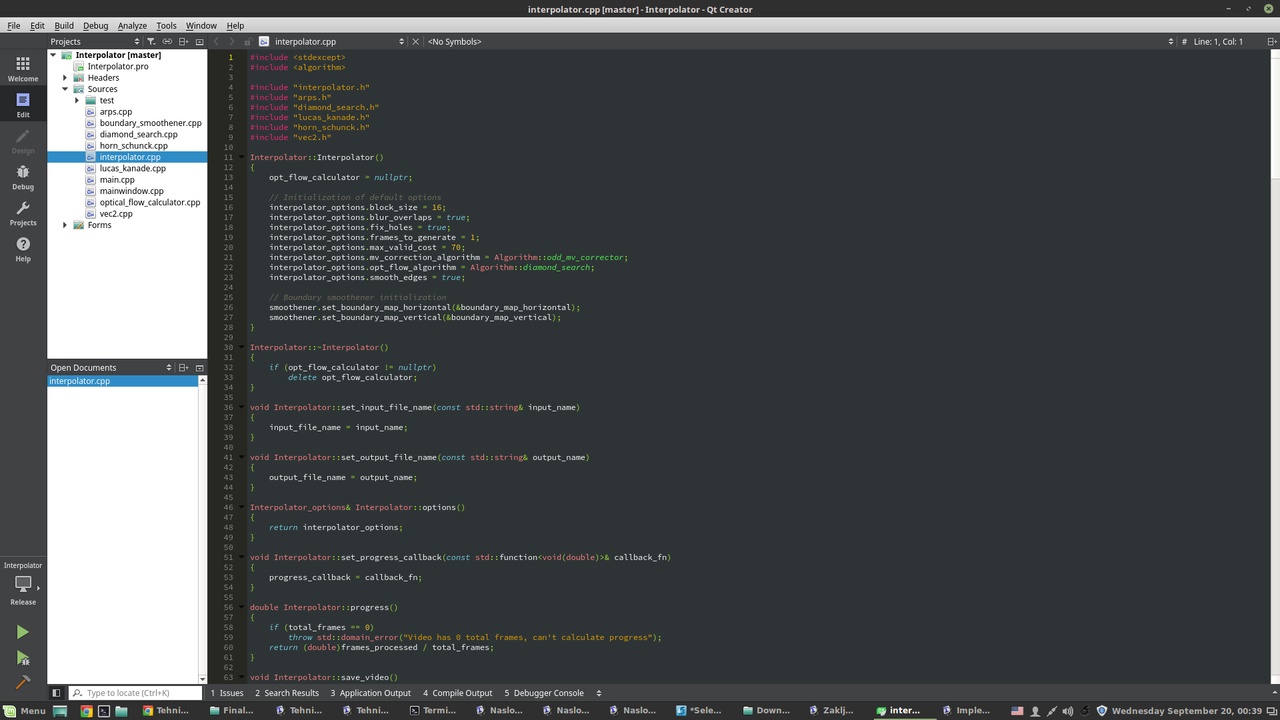
\includegraphics[scale=0.35]{qtscr1}
\centering
\end{figure}

Kod za izbor datoteke kori\sh tenjem QFileDialog klase:
\begin{lstlisting}
std::string input_file = QFileDialog::getOpenFileName(this, "Open video file", "/home/muhamed/Desktop/videos", "All files (*.*)").toStdString();
\end{lstlisting}

Osim raznih GUI kontrola, Qt tako\dj nudi klase i funkcije za HTTP zahtjeve, multimediju, unit testove i druge funkcionalnosti. Osim C++-a, mogu\cj je tako\dj er koristiti QML (\textit{Qt Modeling Language})
za kreiranje GUI aplikacija \cite{qtabout}. QML je jednostavniji jezik od C++-a, me\dj utim C++ je preporu\ch en za pisanje intenzivnijih i slo\zh enijih komponenti aplikacije. Qt tako\dj er ima posebne tipove
podataka koji su namijenjeni da budu kori\sh teni umjesto tipova iz C++ standardne biblioteke, poput \lstinline{QString} i \lstinline{QList}, koje su bolje integrisane sa Qt framework-om od standardnih tipova 
i nude dodatne funkcionalnosti.

Qt je tako\dj er popularan izbor za razvoj mobilnih aplikacija jer ve\cj ina napisanog koda mo\zh e biti biti kori\sh tena na bilo kojoj podr\zh anoj platformi.

\section{Rezultati interpolacije}
Sada \cj emo pogledati nekoliko frejmova jedne video sekvence preuzete sa web stranice youtube.com\cite{examplevideo}. 
Dimenzije kori\sh tenog video zapisa su 1280x720 piksela, a framerate iznosi 24 fps.
Interpolator je koristio algoritam dijamantne pretrage za tra\zh enje opti\ch kog toka, te je izme\dj u svaka dva frejma generisan jo\sh\ jedan:

\begin{figure}[H]
\caption{Prethodni frejm}
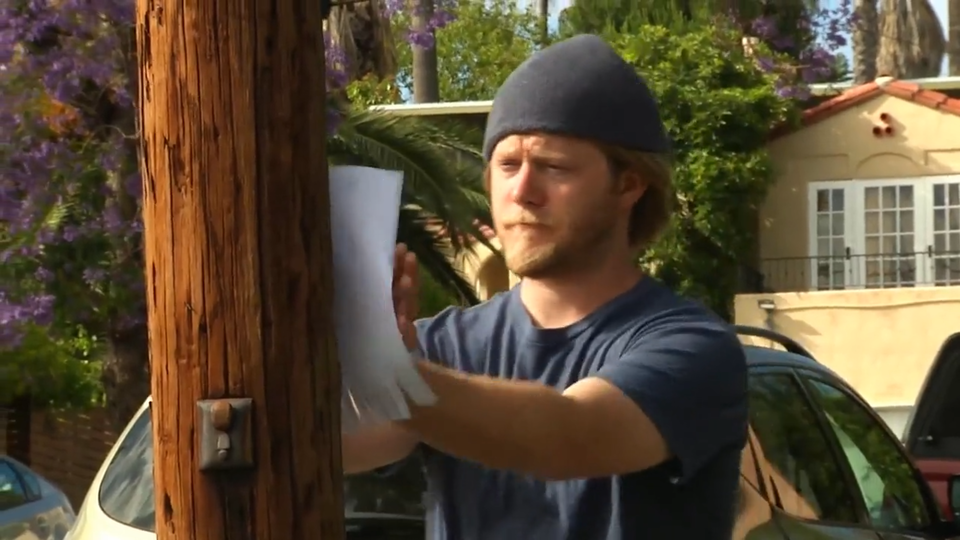
\includegraphics[scale=0.4]{Frame1_s}
\centering
\end{figure}

\begin{figure}[H]
\caption {Interpolirani frejm}
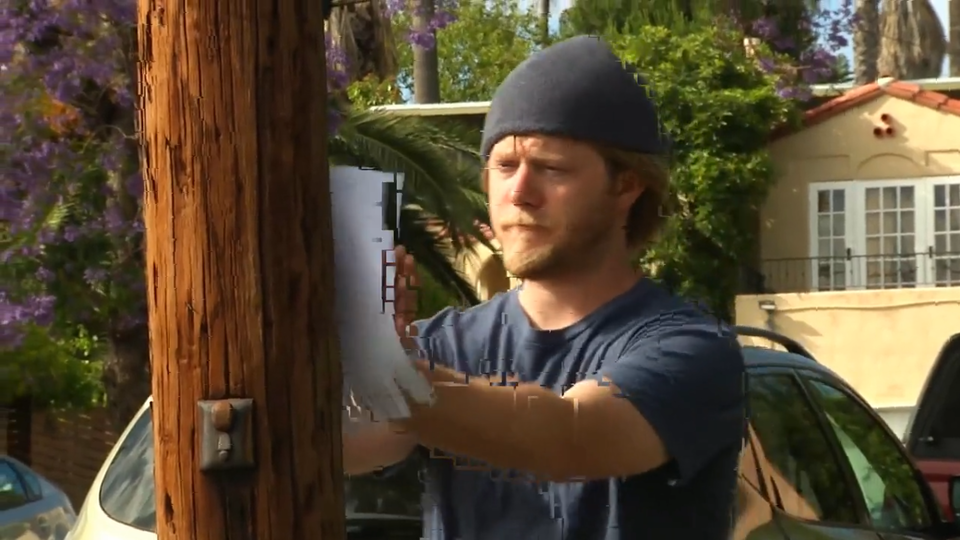
\includegraphics[scale=0.4]{Frame2_s}
\centering
\end{figure}

\begin{figure}[H]
\caption{Naredni frejm}
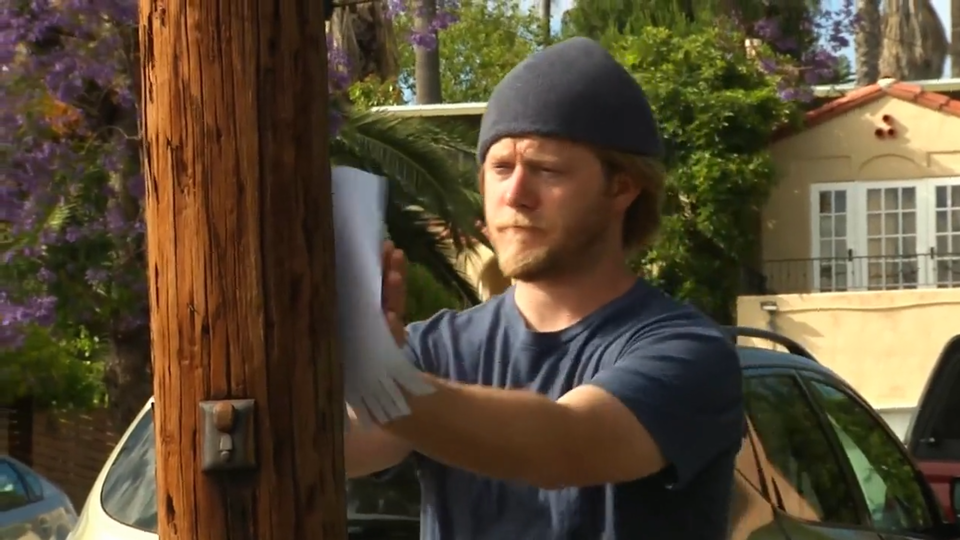
\includegraphics[scale=0.4]{Frame3_s}
\centering
\end{figure}

Prvo \sh to je uo\ch ljivo u interpoliranom frejmu jesu mnogobrojne horizontalne i vertikalne linije. To su artefakti koji su rezultat kori\sh tenja jednostavnog algoritma za interpolaciju. Iako su vektori
pomaka prili\ch no ta\ch ni, jednostavnim "lijepljenjem" blokova (koji su u ovom slu\ch aju veli\ch ine 16x16 piksela) \cj emo uvijek dobiti ovakve artefakte. Da bismo to popravili, morali bismo koristiti
naprednije metode za interpolaciju ili zna\ch ajno pobolj\sh ati algoritam izgla\dj ivanja ivica, koji treba minimizirati upravo ove artefakte. Na interpoliranom frejmu, sa desne strane papira, tako\dj er
mo\zh emo primijetiti da je interpolator ispravno zaklju\ch io da se ti blokovi kre\cj u prema lijevo (jer se papir kre\cj e prema lijevo), te su zbog toga uklonjeni neki pikseli bijelog papira i zamijenjeni
pikselima pozadine. Algoritam je tako\dj er ispravno zaklju\ch io da se ve\cj ina blokova ne pomjera izme\dj u dva frejma, zbog \ch ega su artefakti lokalizovani na dijelove frejma koji se mijenjaju.

Jo\sh\ jedan primjer istog efekta mo\zh emo vidjeti na sljede\cj a tri frejma:

\begin{figure}[H]
\caption{Prethodni frejm}
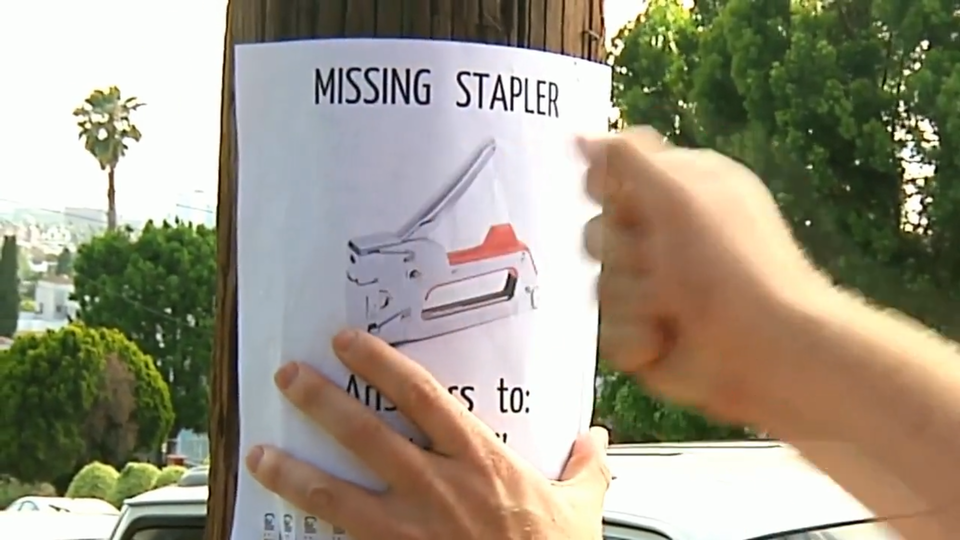
\includegraphics[scale=0.4]{Frame9_s}
\centering
\end{figure}

\begin{figure}[H]
\caption{Interpolirani frejm}
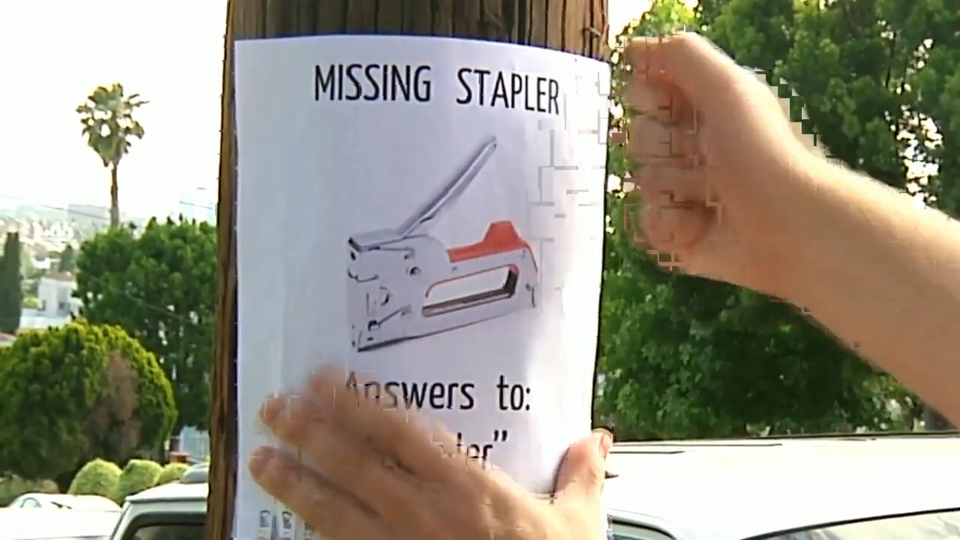
\includegraphics[scale=0.4]{Frame10_s}
\centering
\end{figure}

\begin{figure}[H]
\caption{Naredni frejm}
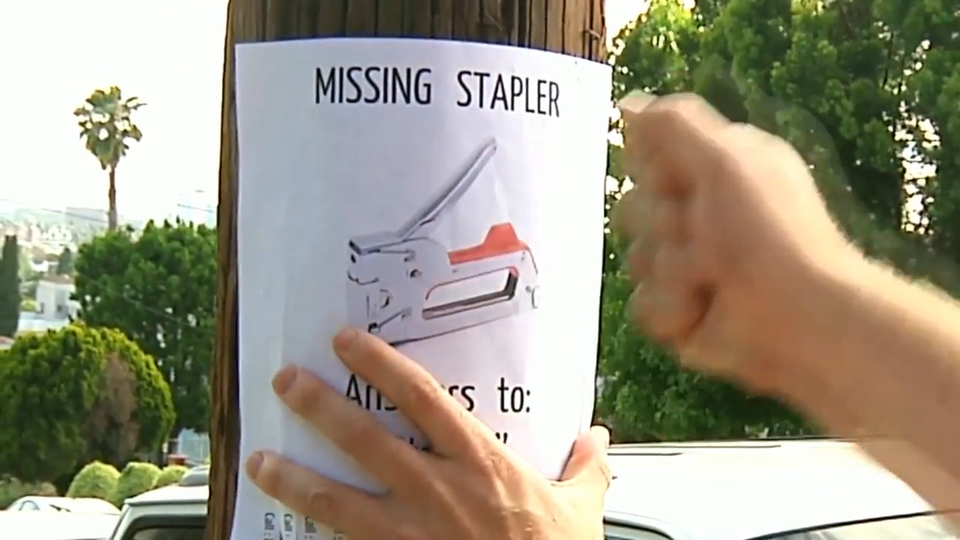
\includegraphics[scale=0.4]{Frame11_s}
\centering
\end{figure}

Na narednom frejmu vidimo \sh ta se desi ako poku\sh amo generisati novi frejm prije keyframe-a, odnosno kada prethodni i naredni frejm nisu sli\ch ni:

\begin{figure}[H]
\caption{Neuspjeli poku\sh aj interpolacije}
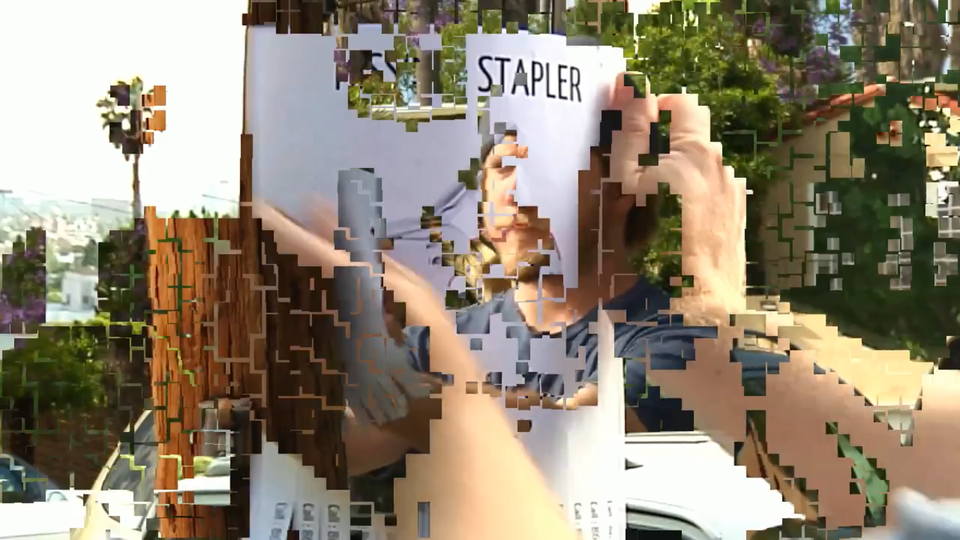
\includegraphics[scale=0.4]{Frame4_s}
\centering
\end{figure}